\documentclass[preprint,5p,times,authoryear]{elsarticle}

\usepackage{wrapfig}
\usepackage[font=small]{caption}
\usepackage[hyperref,usenames,svgnames,dvipsnam]{xcolor}
\usepackage[labelformat=empty]{subcaption}
\usepackage{amsmath}
\usepackage{mathtools}
\usepackage{bm}
\usepackage{breqn}
\usepackage{geometry}
%\usepackage{url}
\usepackage{booktabs}
\usepackage{multirow}
%\usepackage{stfloats}
\usepackage{xfrac}
\usepackage{units}
\usepackage{tabularx}
\usepackage{dblfloatfix}

\usepackage{array}
\newcolumntype{P}[1]{>{\centering\arraybackslash}p{#1}}
\newcolumntype{M}[1]{>{\centering\arraybackslash}m{#1}}

\usepackage{siunitx}
\sisetup{separate-uncertainty}%,range-units = single}
\DeclareSIUnit\year{yr}

\usepackage[colorlinks]{hyperref}

\bibliographystyle{model2-names}\biboptions{authoryear}

\journal{Icarus}

\begin{document}

\hypersetup{
     allcolors = MidnightBlue
}

\urlstyle{same}

\begin{frontmatter}

\title{Numerically Modelling Ocean Dissipation in Titan and Enceladus: A Comparison of Rayleigh and Bottom Drag}

\author[label1]{Hamish C. F. C. Hay\corref{cor1}}
\ead{hhay@lpl.arizona.edu}
\author[label1]{Isamu Matsuyama}
\address[label1]{Lunar and Planetary Laboratory, University of Arizona, Tucson, AZ 85719, United States}

\cortext[cor1]{Corresponding author}

\begin{keyword}
Satellites \sep Ocean Tides \sep Bottom drag\sep Titan \sep Enceladus 
\end{keyword}

\begin{abstract}

Icy satellites that contain subsurface oceans require sufficient thermal energy to prevent the liquid portion of their interiors from freezing. We develop a numerical model to solve the Laplace Tidal Equations on a sphere in order to model tidal flow and thermal energy dissipation in these oceans, neglecting the presence of an icy lid. The model is applied to Titan and Enceladus, where we explore how Rayleigh (linear) and bottom (quadratic) drag terms affect dissipation. The latter drag regime can only be applied numerically. We find excellent agreement between our results and recent analytical work. Obliquity tide Rossby wave resonant features become independent of ocean depth under the bottom drag regime for thick oceans. We show that for Titan, dissipation associated with this Rossby wave resonance acts to dampen the rate of outward orbital migration. Gravity wave resonances can act to cause inward migration, although this is unlikely due to the thin oceans required to form such resonances. Eccentricity tides on Enceladus can provide significant ocean dissipation at resonant gravity-wave resonances, but are also unlikely to do so as thin oceans are required to form these resonances.

\end{abstract}
\end{frontmatter}

\newpage
\section{Introduction}

\hbadness=10000
\vbadness=10000

Thermal energy in the interiors of outer Solar System icy satellites is supplied primarily by radiogenic decay and tidal dissipation. Radiogenic decay plays a role in large icy satellites with a significant portion of silicate material in their interiors \citep{hussmann2006subsurface}. This role, however, diminishes with decreasing mass of silicate material. Small satellites have a high surface area to volume ratio, and consequently thermal energy generated from radioactive decay is lost on a timescale much less than the age of the Solar System. Yet, several small and medium sized icy satellites have confirmed global oceans, suggesting greater interior heating than that provided by radiogenic decay alone.

%Europa exhibits an induced magnetic field consistent with a global layer of salty, liquid water beneath its surface, as measured by the Galileo spacecraft \citep{zimmer2000subsurface, kivelson2000galileo, hand2007empirical}. This is also the case with Ganymede and Callisto, although these liquid oceans are likely to exist at least a few hundred kilometers beneath their surface \citep{zimmer2000subsurface, kivelson2000galileo}. 

This work focuses on Titan and Enceladus. Several interior models and lines of evidence suggest Titan contains a subsurface ocean \citep{sohl2003interior, bills2011rotational, iess2012tides, baland2014titan, mitri2014shape, sohl2014structural}. Enceladus also shows strong evidence of a liquid ocean beneath its surface. Originally it was thought that this liquid reservoir was localised beneath the South Polar Terrain (SPT) of the satellite \citep[e.g.,][]{collins2007enceladus}. However, recent modelling of the degree-2 gravity field was consistent with a global ocean with greatest thickness beneath the SPT, although such models are non-unique \citep{iess2014gravity,mckinnon2015effect}. Most recently, the large forced libration of Enceladus indicates a decoupling of the icy shell from its interior, and thus the presence of an ocean of global extent \citep{thomas2016enceladus}.  

%Tidal dissipation is currently considered the most promising mechanism to provide energy to heat these oceans over geological timescales, and shall be the main focus of this paper.

\textbf{This paper is intended to introduce and verify a new numerical model for solving thin shell ocean dynamics in planetary bodies. The model is therefore ideal for investigating ocean dissipation in a variety of icy satellites. Assumptions made in the development of the numerical code reflect those made in the semi-analytical models to which our results are compared. This ensures the most accurate validation of the numerical model. We also introduce bottom drag into the model, an extension that is only possible numerically and in simplified scaling analysis \citep{chen2013tidal}. We explore this drag regime for oceans on Titan and Enceladus.}

\subsection{Tidal Dissipation}

Any satellite that passes through a varying gravitational potential will experience some form of tidal dissipation. The time varying gravitational potential may be a result of the satellite's orbital eccentricity and/or obliquity, as well as any non-synchronous rotation. For a satellite in (near) synchronous rotation, the gravitational tidal potential will vary periodically over the satellite's orbit. The changing potential does mechanical work on the satellite, and a portion of this work is converted to thermal energy. This process is known as tidal dissipation. As long as sufficient orbital or rotational energy remains in the system (in the form of eccentricity, obliquity or non-synchronous rotation), tidal dissipation will occur.

Both the solid and fluid regions of a satellite will experience tidal dissipation. Despite this, and the overwhelming evidence for and abundance of subsurface oceans in the icy satellites, the majority of dissipation studies have focused on only solid-body tides, \citep[e.g.,][]{moore2000tidal, tobie2005tidal,roberts2008tidal, beuthe2013spatial}.
Most terrestrial tidal dissipation occurs within the oceans, and while Earth has a complex dynamic between tidally-induced ocean flow and its continents, it illustrates the importance of considering ocean dissipation.

The effect of ocean dissipation in outer planet satellites was first considered for Titan by \citet{sagan1982tide}, who analytically derived expressions to estimate dissipated energy in a global hydrocarbon surface ocean. In doing so they attempted to explain Titan's relatively high eccentricity. The same problem was then approached numerically by \citet{sears1995tidal}, who solved the Laplace Tidal Equations (LTEs) to derive time averaged estimates of dissipated energy within a hydrocarbon ocean of varying thicknesses. Sears' numerical model is the basis for the model described in this paper.

More recently, \citet{tyler2008strong,tyler2009ocean,tyler2011tidal,tyler2014comparative} has done extensive work on ocean dissipation, showing that thermal energy released by an ocean can theoretically prevent a subsurface liquid from freezing. By exploring how ocean thickness and drag coefficient effect dissipation, \citet{tyler2011tidal} discovered ocean dissipation resonances. These resonances tend to occur for particular ocean thicknesses, where oceanic planetary waves resonantly interact with the periodic tidal forcing, allowing enhanced tidal flow and consequently enhanced tidal dissipation. \citet{matsuyama2014tidal} developed a similar model to that used by \citet{tyler2011tidal}, adding the effects of ocean loading, self-attraction, and deformation of the solid regions. These effects were shown to alter the position and magnitude of these dissipative resonances. \citet{kamata2015tidal} has also modelled the effects of an icy shell on Love number resonances, but did not include any ocean dynamics in their approach.

\citet{tyler2011tidal}, \citet{matsuyama2014tidal}, and \citep{chen2013tidal} all considered Rayleigh (linear) drag in their models.  \citet{chen2013tidal} also developed a set of scaling laws to model ocean dissipation in the bottom (quadratic) drag regime. The numerical model presented in this work is capable of solving the LTEs using both Rayleigh and bottom drag, as is typical in terrestrial ocean dissipation studies \citep{taylor1920tidal,jeffreys1921tidal,zahel1977global,egbert2001estimates,jayne2001parameterizing}. \citet{sears1995tidal} used both Rayleigh and bottom drag simultaneously in his model. In contrast, we adopt a bimodal approach to illustrate the differences between Rayleigh and bottom drag. These two regimes are briefly described below.

\subsection{Rayleigh Drag}

A linear formulation of drag was first introduced as the Guldberg-Mohn approximation of \textit{virtual} internal friction in 1876 \citep{neumann1968ocean}. Now known as Rayleigh drag, the approximation describes drag within a fluid that is proportional and opposite to the fluid's velocity. That is, the drag force per unit mass $\bm{F_d} = -\alpha \bm{u}$, where $\alpha$ is some drag time scale known as the coefficient of Rayleigh drag with units of $\si{\per\second}$. The flow velocity is $\bm{u}$. 

Rayleigh drag can be though of as a macroscopic description of drag between adjacent fluid elements in a moving liquid.

\subsection{Bottom Drag}

Terrestrial ocean dissipation studies often employ a drag model that scales with the square of the fluid's velocity. This quadratic dependence of drag on flow velocity is often referred to as \textit{bottom drag} \citep{gill1982atmosphere}, and arises due to turbulent flow interacting with some bottom boundary, such as the ocean floor. Large tangential shear stresses associated with this interface generate a turbulent boundary layer where there is a significant transfer of momentum from the flow. While such turbulent flow cannot be resolved at the scale of planetary ocean simulations, the bottom drag coefficient $c_D$ is empirically derived to include the frictional effect of this turbulence at the planetary scale.

In this work we investigate the effects of bottom drag on ocean dissipation for both Titan and Enceladus, structuring the paper as follows. Firstly, we introduce our numerical method in section \ref{sec:method}, describing the grid structure and numerical solver as well as its current limitations. Secondly, we then apply this model to both Titan (section \ref{sec:results_Titan}) and Enceladus (section \ref{sec:results_Enceladus}) in turn for each drag model, examining how dissipation differs between each case. The Rayleigh drag results are compared to semi-analytical solutions of \citet{matsuyama2014tidal}. We also compare the bottom drag results against scaling laws developed by \citep{chen2013tidal}.








\section{Methodology}\label{sec:method}

This section describes some of the theory and methods involved in this work. The governing equations of the numerical model are discussed in section \ref{subsec:LTE}. We then provide analytical expressions for the degree-2 tidal potential in section \ref{subsec:pot}. Following this, descriptions of the discretisation and numerical scheme are outlined in section \ref{subsec:model}, with a summary of our simulations ran in section \ref{subsec:param}.

\subsection{Laplace Tidal Equations \label{subsec:LTE}}

The equations of motion and continuity that describe ocean flow in the shallow water limit are known as the Laplace Tidal Equations (LTEs) \citep{lamb1932hydrodynamics}. The main assumption leading to this set of equations is that radial (vertical) ocean flow is negligible when compared to lateral flow, reducing the problem to two dimensions. This is indeed a good approximation at the planetary scale, where lateral flow length scales span much greater distances than the thickness of an ocean. The conservation of mass (eq. \ref{eq:mass}) and momentum (eq. \ref{eq:mom}) that make up the LTEs, including both Rayleigh and bottom drag, are given as \citep{sears1995tidal,tyler2008strong,matsuyama2014tidal}:

%Adds vertical space between equations
%\setlength{\jot}{8pt}
%environment centres all equations

\vspace{-0.5cm}
\begin{gather}
\partial_t \eta + \nabla \cdot \left(h \bm{u}\right) = 0\, , \label{eq:mass}\\
\begin{aligned} 
\partial_t \bm{u} + 2 \bm{\Omega} \times \bm{u} + \alpha\bm{u} + \frac{c_D}{h} \left|\bm{u}\right| \bm{u}  + g \nabla \eta = (1 + k_2 - h_2) \nabla U_2 \, . \label{eq:mom}\\
\end{aligned} 
\end{gather}

Equation \ref{eq:mass} consists of two terms. The first is the time rate of change of vertical sea surface displacement, $\eta$, about some equilibrium level, $h_0$, where the total ocean thickness, $h = h_0 + \eta$. The second term is the divergence of the ocean thickness multiplied by the surface velocity vector, $\bm{u} \equiv (u, v)$, where $u$ and $v$ are the eastward and northward velocity components, respectively. This divergence term is required to conserve mass.

The term on the right hand side of Equation \ref{eq:mom} is an applied force per unit mass. $\nabla U_2$ is the gradient of the degree-2 tide raising potential, discussed in section \ref{subsec:pot}. It is multiplied by Love's reduction factor, $1 + k_2 - h_2$. Love's first number, $k_2$, is a proportionality constant accounting for the additional tidal potential due to the elastic redistribution of mass on the satellite. $h_2$, the second Love number, accounts for the tidal potential arising from solid body surface displacement of the satellite \citep{love1911some}.

The time derivative of velocity is the first term on the left hand side of the momentum equation (eq. \ref{eq:mom}). It is balanced by four force per unit mass terms on the left. The first of these terms is the coriolis acceleration, where $\bm{\Omega}$ is the satellite's rotational angular velocity vector. Rayleigh and bottom drag are described in the next two terms, where $\alpha$ and $c_D$ are the Rayleigh and bottom drag coefficients, respectively \citep{sears1995tidal,chen2013tidal}. The last term on the left hand side of Equation \ref{eq:mom} is the gravitational restoring acceleration per unit mass. It acts to restore changes in sea surface displacement about the undisturbed ocean thickness, $h_0$. \textbf{As displacements are small with respect to the ocean thickness ($\eta \ll h_0$),  Equations \ref{eq:mass} and \ref{eq:mom} simply become,  }

\vspace{-0.5cm}
\begin{gather}
\partial_t \eta + h_0 \nabla \cdot \bm{u} = 0\, , \label{eq:mass_lin}\\
\begin{aligned} 
\partial_t \bm{u} + 2 \bm{\Omega} \times \bm{u} + \alpha\bm{u} + \frac{c_D}{h_0} \left|\bm{u}\right| \bm{u}  + g \nabla \eta = (1 + k_2 - h_2) \nabla U_2 \, , \label{eq:mom_lin}\\
\end{aligned} 
\end{gather}

\noindent \textbf{respectively.} \textbf{The assumption that $\eta \ll h_0$ is valid over much of the parameter space explored in sections \ref{sec:results_Titan} and \ref{sec:results_Enceladus}. However, as the ocean thickness approaches gravity-wave resonant configurations, this assumption breaks down. A more rigorous approach would instead solve equations \ref{eq:mass} and \ref{eq:mom} directly. Without such an assumption, the maximum ocean displacement would likely be reduced, limiting (but not removing) the dissipative nature of gravity-wave resonances. The small displacement assumption has been made in this work in order to verify the numerical model against the semi-analytical solutions of \citet{matsuyama2014tidal}. The assumption linearises the problem, which is necessary for the semi-analytical models from \citet{tyler2011tidal} and \citet{matsuyama2014tidal}. In future work this shall be addressed.}      

\subsection{\textbf{Applicability of the Laplace Tidal Equations} \label{subsec:applicability}}

\textbf{Some discussion of how readily the LTEs can be applied to icy satellites is required. Clearly, no icy satellite contains a global or near-global surface ocean of any kind. Instead, all oceans in the Solar System, with the exception of Earth, are located beneath an ice shell. As the thickness of the ice shell increases the overburden pressure on the ocean also increases. Additionally, the rigidity of the shell will also increase. Both of these will limit the ability to which a subsurface ocean can respond to an applied tidal forcing. As such, we can consider the results presented in this paper as upper limits to the amount of possible energy dissipation through the action of surface gravity-waves. However, for thin ice shells ($<\SI{10}{\kilo\metre}$) (can we do an OOM calculation here?) the ability of the solid lid to resist changes in the ocean surface is small, and we would still expect the ocean surface to respond to the tidal forcing, albeit in a dampened manner.}   

\textbf{As mentioned by \citet{tyler2008strong}, ocean dynamics are not purely expressed through changes in ocean surface height and gravity-waves. Another class of ocean oscillation, the Rossby-wave, is expected to develop as a result of coriolis forces acting on the flow in the rotating reference frame. There is no lateral divergence associated with this type of flow, so no changes in ocean surface height develop. This type of flow can readily exist under a thick and rigid ice shell. It is therefore useful, while not perfectly accurate, to investigate ocean dissipation in icy satellites using the numerical model described here where we assume a surface ocean. Additionally, there are situations where assuming a surface ocean is appropriate. For example, tidal dissipation in the magma oceans of the proto-Earth and proto-Moon played a large role in the thermal and orbital evolution of those bodies, as recently explored by \citet{chen2016tidal}.}

\textbf{The intention of this paper is to provide a stepping stone for further development of this model by incorporating an ice shell into our code. Assuming a surface ocean is a natural place to begin.}


\subsection{Tidal Potential \label{subsec:pot}}

Finite eccentricity and obliquity cause libration of the satellite's tidal bulge in longitude and latitude, respectively. It is this libration that primarily induces ocean flow. We therefore find it convenient to split the time-dependent degree two tidal potential into two main components, the eccentricity and obliquity tides:

\begin{align}
U_2 &= U_{ecc} + U_{obliq}\, . \label{eq:U_2}
\end{align}

To first order in eccentricity and obliquity, the two primary tidal components can be expressed as \citep{tobie2005tidal,tyler2011tidal},

\begin{equation}
U_{ecc} = \Omega^2 R^2 e \left\lbrace - \frac{3}{2} P_{20}\left(\cos\theta\right) \cos \left(\Omega t \right) + \frac{1}{8} P_{22}\left( \cos\theta\right) \right. \\ 
\times \left. \vphantom{\frac{1}{8}} \left[7 \cos \left(2 \phi - \Omega t \right) - \cos \left(2 \phi + \Omega t\right) \right] \right\rbrace, \label{eq:U_ecc}
\end{equation} and,

\begin{equation}
U_{obliq} = \frac{1}{2}\Omega^2 R^2 \theta_0 P_{21}\left(\cos\theta\right)\\
\times \left[ \cos \left(\phi - \Omega t \right) - \cos \left( \phi + \Omega t\right) \right] \, ,\label{eq:U_obliq}
\end{equation}

where $r$ is the satellite's radius, $e$ is its eccentricity, and $\theta_0$ is the obliquity in radians. Co-latitude and longitude are given as $\theta$ and $\phi$ respectively. $P_{lm}$ represents the associated Legendre function of degree $l$ and order $m$. The eccentricity tide can be further split into the two terms on the right hand side of Equation \ref{eq:U_ecc}. These terms represent the eccentricity-radial ($U_{20}$) and eccentricity-libration ($U_{22}$) tides respectively, as described by \citet{tyler2011tidal}. We can therefore rewrite equation \ref{eq:U_2} as $U_2 = U_{20} + U_{21} + U_{22}$.

\begin{figure}[t]
\centering
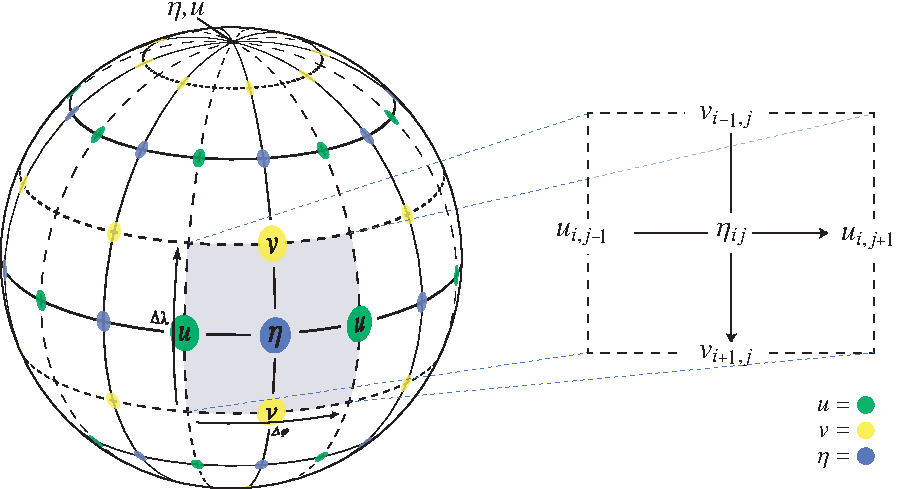
\includegraphics[width=0.8\linewidth]{Figures/GridDiagram_revision}
\caption{The staggered grid structure used in ODIS. A single cell is show on the right of the figure, where surface displacement, $\eta$, represents a cell centered quantity. $u$ velocity nodes are staggered eastward of $\eta$, whereas $v$ velocity nodes are staggered southwards. Both $u$ and $v$ are defined at the cell walls. Lines of meridian merge to singularities at the poles, where a single $\eta$ and multiple $u$ nodes are stored.\label{fig:grid}}
\end{figure}

\subsection{Tidal Quality Factor}

A useful parameter for understanding tidal dissipation is the quality factor, $Q$. Defined as the ratio of maximum energy stored to the total energy dissipated in a purely elastic body, small values of $Q$ correspond to a dissipative environment \citep{goldreich1966q}. \citet{tyler2011tidal} and \citet{matsuyama2014tidal}, however, use the kinetic energy $E_k$ of the fluid system to represent the energy stored in the tide;

\begin{equation}\label{eq:Q}
Q \equiv 2 \pi \dfrac{\text{max} \left( E_{k} \right)}{E_{diss}} = \dfrac{\Omega}{2 \alpha}
\end{equation}

where the total time averaged dissipation is $E_{diss}$. This definition is ill-defined, however, as the the kinetic and dissipated energy in the ocean tide are intrinsically coupled. Large drag coefficients enhance dissipation, but this demands a decrease in the kinetic energy of the system, which in turn results in a reduction in velocities and consequently dissipation. This coupling makes it difficult to use a definition of $Q$ that is meaningful to the Planetary Science community. We suggest that a more appropriate definition would be using the maximum stored energy in the equilibrium tide (i.e., the theoretical instantaneous tide raised in the absence of dissipation) in the numerator of Equation \ref{eq:Q}, which is used in dissipation studies of gas planets \citep{goldreich1966q}. For the remainder of this work, however, we return to simply presenting our results as a function of drag coefficient, rather than potentially misleading readers with alternate definitions of $Q$. 

\subsection{Numerical Model \label{subsec:model}}

In this section we outline our two dimensional, finite difference computational fluid dynamics (CFD) model, known as Ocean Dissipation in Icy Satellites (ODIS). In its current form, ODIS is based extensively on the models discussed in and developed by \citet{zahel1973diurnalk,zahel1978influence} and \citet{sears1994tidal,sears1995tidal}. We first provide a description of the numerical grid. An overview of the finite difference scheme itself is then given, before summarising and illustrating limitations of the finite difference scheme and grid choice.

\subsubsection{Discretized Grid \label{subsec:grid}}

We employ a fixed latitude-longitude grid for our numerical simulations, defined in a spherical coordinate system. The grid is constructed in a staggered manner, meaning that velocity nodes are placed to the east and south of their parent displacement nodes. \textbf{This is identical to the Arakawa ``C'' grid introduced by \citet{arakawa1977computational}}. This is illustrated in Figure \ref{fig:grid}, where we define $u$ and $v$ as the eastward and northward velocity components, respectively. $\Delta \lambda$ is the grid spacing in latitude, whereas $\Delta \phi$ is the grid spacing in longitude. A staggered approach is adopted as it avoids numerical oscillations that grow in the solution by calculating derivatives \textit{between} grid nodes rather than over them. This is discussed further in section \ref{subsec:fd_expan}.

As is clear from Figure \ref{fig:grid}, lines of meridian all converge to single points at either pole. Consequently, the model is forced to go from $m$ longitudinal grid points immediately surrounding the pole to merely a single point at the pole itself. Accordingly, single values of $\eta$ are stored at each pole, whereas multiple $u$ values are required to maintain numerical stability. 

ODIS stores three separate 2D arrays for $\eta$, $u$ and $v$. They are accessed in a parent-child configuration, whereby the velocity nodes immediately east and south of a displacement node are the children to their parent $\eta$. Both $u$ and $v$ at the southern and eastern walls of the cell in Figure \ref{fig:grid} are children to the central $\eta$ node. % This is of little importance to the model's computations, but does lend some insight into the infrastructure of ODIS.

\subsubsection{Finite Difference Expansions \label{subsec:fd_expan}}

In order to solve the LTEs, we expand equations \ref{eq:mass_lin} and \ref{eq:mom_lin} in a semi-implicit finite difference scheme in spherical coordinates \citep{sears1995tidal}. \textbf{Details of the coordinate transform for these equations are given in \ref{app:coords}.} Expanding $\bm{u}$ into its components and assuming $\eta \ll h_0$, the momentum equation becomes,

\vspace{-0.6cm}
\begin{equation}
u_{ij}^{t+1} \approx  \left[ \,2 \Omega \bar{v}_{ij}^{\textbf{t}} \sin{\lambda_i} \vphantom{\frac{c_D}{h_0}\sqrt{\left(u_{ij}^{t}\right)^2}} - \alpha u_{ij}^{t} \right. \\ 
- \frac{c_D}{h_0}\sqrt{\left(u_{ij}^{t}\right)^2 + \left(\bar{v}_{ij}^{t}\right)^2}\cdot u_{ij}^{t} - \frac{g}{R \cos{\lambda_i}} \frac{\partial \eta_{ij}^{t}}{\partial \phi_j} \\  
+ \left.\left(1 + k_2 - h_2\right) \frac{1}{R \cos{\lambda_i}} \frac{\partial U_{2,ij}^{t}}{\partial \phi_j} \right]  \Delta t + u_{ij}^{t} \, , \label{eq:momu_fd}
\end{equation}
\vspace{-0.6cm}
\begin{equation}
v_{ij}^{t+1} \approx  \left[ \,-2 \Omega \bar{u}_{ij}^{\textbf{t}} \sin{\lambda_i} \vphantom{\frac{c_D}{h}\sqrt{\left(u_{ij}^{t}\right)^2}} - \alpha v_{ij}^{t} \right. \\ 
- \frac{c_D}{h_0}\sqrt{\left(\bar{u}_{ij}^{t}\right)^2 + \left(v_{ij}^{t}\right)^2}\cdot v_{ij}^{t} - \frac{g}{R} \frac{\partial \eta_{ij}^{t}}{\partial \lambda_i} \\  
+ \left.\left(1 + k_2 - h_2\right) \frac{1}{R} \frac{\partial U_{2,ij}^{t}}{\partial \lambda_i} \right]  \Delta t + v_{ij}^{t} \, , \label{eq:momv_fd}
\end{equation}

\noindent and the continuity equation becomes, 

\begin{equation}
\eta_{ij}^{t+1} \approx 
-\frac{h_0}{R \cos{\lambda_i}}\left[
\frac{\partial \left(v_{ij}^{t+1} \cos{\lambda_i}\right)}{\partial	\lambda_i}  
+\frac{\partial u_{ij}^{t+1}}{\partial	\phi_j}\right]
\Delta t
+ \eta_{ij}^{t}\, . \label{eq:mass_fd}
\end{equation}

Latitude and longitude are denoted by $\lambda$ and $\phi$ respectively. $i$ and $j$ represent the $i\text{th}$ and $j\text{th}$ latitude and longitude nodes within the grid. The time index is given by $t$, and $\Delta t$ represents the time-step. Overbars correspond to spatial averages, a necessity given the staggered nature of the grid. Spatial and temporal expansions are made using the Euler method and are first order accurate in space and time.

All derivatives of the degree-2 tidal potential (equations \ref{eq:U_ecc} and \ref{eq:U_obliq}) have analytical solutions, and thus do not require further finite difference expansion. Derivatives of all other quantities, however, do require further expansion. The expansions take the general form of either,

\begin{align}
\frac{\partial w_{ij}^{\textbf{t}}}{\partial \lambda} &\approx \frac{w_{i+\nicefrac{1}{2},j}^{\textbf{t}} - w_{i-\nicefrac{1}{2},j}^{\textbf{t}}}{\Delta \lambda} \, , \label{eq:gen1}
\end{align} or,

\begin{align}
\frac{\partial w_{ij}^{\textbf{t}}}{\partial \phi} &\approx \frac{w_{i,j+\nicefrac{1}{2}}^{\textbf{t}} - w_{i,j-\nicefrac{1}{2}}^{\textbf{t}}}{\Delta \phi} \, , \label{eq:gen2}
\end{align}

\noindent where $w$ represents $u$, $v$ or $\eta$.

Equations \ref{eq:gen1} and \ref{eq:gen2} show that each derivative is evaluated halfway between the nodes where $w$ is stored. Consequently, any derivative of $w$ is calculated at a position held by a different variable because the grid is staggered. For example, $\partial_\phi u_{ij}$ is always evaluated at the position held by $\eta_{ij}$ as $u_{i,j-\nicefrac{1}{2}}$ and $u_{i,j+\nicefrac{1}{2}}$ lie to the left and right of $\eta_{ij}$,  respectively. This is shown clearly on the right of Figure \ref{fig:grid}.

\subsubsection{Numerical Scheme}

ODIS begins its calculations by (1) determining the mass of each volume element in the initial ocean assuming an undisturbed ocean of thickness $h_0$. With the mass calculated in each cell, it is then possible to find the dissipated energy in the system.

The next step in the numerical integration is to calculate $\nabla U_2$ across all $u$ and $v$ grid points (2). This gives the initial force per unit mass experienced by a fluid element in the model domain.

Once the tidal acceleration is known, ODIS directly calculates $u$ and $v$ over the grid by solving equations \ref{eq:momu_fd} and \ref{eq:momv_fd} (3). This step is purely explicit as $u$ and $v$ depend only on information from the previous time step, $t$. Following this, $\eta$ is then updated using the new velocity values (4). In contrast to the velocity calculations, this step is semi-implicit as it relies on values from both the current and previous time steps, as shown in Equation \ref{eq:mass_fd} \citep{sears1995tidal}.

After solutions for $u$, $v$, and $\eta$ are found at the new time step, $t+1$, the energy calculations begin (5). For Rayleigh drag, ODIS calculates and stores global dissipated energy flux as,

\begin{equation}
F_{\alpha}^{t+1} = \frac{1}{4 \pi R^2 }\sum_{i=1}^{n} \sum_{j=1}^{m} \alpha \textbf{M}_{ij} \left[\left(u_{ij}^{t+1}\right)^2 + \left(v_{ij}^{t+1}\right)^2\right] \, , \label{eq:E_alpha}
\end{equation}

for $n$ and $m$ grid points in latitude and longitude, respectively. The summed terms in Equation \ref{eq:E_alpha} give the total dissipated energy in the system across the current time step, \textbf{for the total ocean column mass $\textbf{M}$ within each cell}. The factor in front of the summations then averages this quantity over the satellite's surface area giving $F_{\alpha}$ in watts per square metre. For bottom drag the equivalent expression is

\begin{equation}
F_{c_D}^{t+1} = \frac{1}{4 \pi h_0 R^2 }\sum_{i=1}^{n} \sum_{j=1}^{m} c_D M_{ij} \left[\left(u_{ij}^{t+1}\right)^2 + \left(v_{ij}^{t+1}\right)^2\right]^{\nicefrac{3}{2}}\, . \label{eq:E_cd}
\end{equation}

Every time step calculations 2-5 are repeated, beginning with determining $\nabla U_2$. Finally, at the end of each orbit, $F_\alpha$ or $F_{c_D}$ is summed and averaged over the orbital period (6). This gives the time and surface averaged heat flux due to tidal dissipation for Rayleigh drag,

\begin{align}
\left\langle F_\alpha \right\rangle_{orbit} &= \frac{1}{p}\sum_{t=1}^{p} F_{\alpha}^{t}  \, , \label{eq:E_alpha_orbit}
\end{align} 
and bottom drag,

\begin{align}
\left\langle F_{c_D} \right\rangle_{orbit} &= \frac{1}{p}\sum_{t=1}^{p} F_{c_D}^{t}  \, , \label{eq:E_cd_orbit}
\end{align}

where $p = \nicefrac{T}{\Delta t}$, the total number of time steps in the orbital period, $T$. These expressions are consistent with \citet{sears1995tidal}.

Steps 2-6 are repeated until the model has converged into a periodic equilibrium. Care must be taken when selecting convergence criteria. Simulations involving thick oceans and small drag coefficients will oscillate about their converged solution with periods of \numrange{10}{100} orbits or more due to the large inertia associated with thick, poorly dissipative oceans (see Figure \ref{fig:conv_a}). These simulations clearly require longer run-time. For the most time consuming simulations, we take the mean dissipation over one full oscillatory cycle.

\begin{figure}
\centering
\includegraphics[width=0.85\linewidth]{Figures/spatial_error_ecc}
\caption{\textbf{Displacement solutions (left column) and corresponding percentage error (right column) for Enceladus' eccentricity tide with $h_0 = \SI{500}{\metre}$ and $\alpha = \SI{e-5}{\per\second}$. The numerical grid was spaced at \SI{1}{\degree}. Each row corresponds to a different time interval throughout one orbital period, $T$. Percentage eror is  $< \SI{0.01}{\percent}$ over much of the model domain, with local highs where the solution passes from postive to negative displacement.} \label{fig:spatial_error}}
\end{figure}


\subsubsection{\textbf{Numerical Tests} \label{subsubsec:num_test}}

As with any numerical solution there are errors associated with discretisation of the problem into the model domain. We performed resolution testing across various ocean thicknesses to determine how these errors scale with grid resolution \textbf{using the semi-analytical solutions of \citet{matsuyama2014tidal} as our benchmark in all following numerical tests. Although the solutions from \citet{matsuyama2014tidal} are not purely analytical, we use solutions that are truncated at spherical harmonic degree $l=20$. As such, these can be considered the exact solutions. Four of these tests are shown in this section to illustrate that the numerical method and code perform as expected, both as a function of space and time. Each test shown here was run for Enceladus' eccentricity tide, using $h_0 = \SI{500}{\metre}$, $\alpha = \SI{e-5}{\per\second}$, and $\Delta t = \SI{2}{\second}$. The grid was spaced at \SI{1}{\degree} throughout, except in tests 3 and 4 which examine how the numerical error depends on model resolution.}

\begin{figure}[t]
\centering
\includegraphics[width=\linewidth]{Figures/temporal_error_ecc}
\caption{\textbf{Normalised error norms as a function of time for Enceladus' eccentricity tide with $h_0 = \SI{500}{\metre}$ and $\alpha = \SI{e-5}{\per\second}$. At approximately \num{10} orbits, all parts of the solution have converged after which the normalised error remains small, and oscillates over the orbital period.} \label{fig:temporal_error}}
\end{figure}


\begin{figure}[t]
\centering
\includegraphics[width=0.6\linewidth]{Figures/convergence_eta}
\caption{\textbf{Normalised error norms as a function of time for Enceladus' eccentricity tide with $h_0 = \SI{500}{\metre}$ and $\alpha = \SI{e-5}{\per\second}$, taken at pericenter at the beginning of orbit \num{100}. A least-squares fit to each error norm in log-log space yields slopes of \num{0.86}, \num{0.90} and \num{1.03} for the $L_1$, $L_2$ and $L_{\infty}$ normalised error norms, respectively.} \label{fig:spatial_convergence}}
\end{figure}



\begin{figure*}[!t]
    \centering
    \begin{subfigure}[t]{\linewidth} % contains the two plots in a single figure
        \includegraphics[width=\linewidth]{Figures/convergence2}
        \phantomcaption
        \label{fig:conv_a}
    \end{subfigure}
    \begin{subfigure}[t]{0\linewidth} % the hidden unwanted image
         \includegraphics[width=\linewidth]{Figures/convergence2}
         \phantomcaption
         \label{fig:conv_b}   
    \end{subfigure}
    \vspace{-0.5cm}
\caption{Dissipation convergence and error scaling as a function of grid resolution. Panel \ref{fig:conv_a} shows the time evolution of the orbit-averaged dissipated energy at periapsis. The solid lines represents different grid resolutions, whereas the dashed line is the semi-analytical solution for Rayleigh drag from \citet{matsuyama2014tidal}. Panel \ref{fig:conv_b} shows the \textbf{dissipation} error between the numerical and semi-analytical solutions with increasing resolution. The least-squares slope of the first six data points (when the slope is steady) in log-log space is \num{1.94}. These simulations are for the obliquity tide using $h_0 = \SI{1}{\kilo\metre}$ and $\alpha = \SI{e-8}{\per\second}$ on Titan. \label{fig:conv}}
\end{figure*}

\textbf{It is important to understand how the model resolves the solution across the numerical domain, especially when using the fixed latitude-longitude grid employed here. This is done in test 1 (Figure \ref{fig:spatial_error}) where the ocean surface displacement (left) is compared to the corresponding error field (right). The ocean configuration is near a gravity-wave resonance, so it is easy to discern the eastward propagating gravity-wave through the model domain at each time slice. Note that at pericentre ($t/T = 0$) positive displacements are at a maximum, while at apocentre ($t/T = 0.5$) they are at a minimum. The percentage error in the numerical model is very small ($< \SI{0.01}{\percent}$) over the majority of the domain. Near the poles, where grid points are closely arranged, numerical error is smallest. At the zero-crossing in displacement both the numerical and semi-analytical solutions become $\ll \SI{1}{\metre}$. As a result, the numerical error locally spikes in those regions producing the rings of high error seen in Figure \ref{fig:spatial_error}. Overall, the numerical error is very low, giving us confidence in the ability of ODIS to spatially resolve the solutions.}  

\textbf{As the tidal forcing in this problem is periodic, one expects the solution and its corresponding error to also be periodic. It is therefore logical to investigate how the numerical error changes over time. We investigate this in our second test, starting the numerical simulations from an undisturbed and unforced ocean. This is shown in Figure \ref{fig:temporal_error}, where once again the numerical error is computed against the \citet{matsuyama2014tidal} semi-analytical solutions. The error is quantified using the normalised $L_1$, $L_2$ and $L_{\infty}$ error norms (defined in \ref{app:error}). The maximum error in each solution if given by the $L_{\infty}$ norm. Normalised error is greatest at the beginning of the simulation, as this is during the model ``spin-up'' time. After approximately \num{10} orbits both the displacement and two velocity solutions converge. At this point the average error over each orbital period remains constant. The magnitude of this converged error is a function of the grid resolution, as shown in test 3. Once converged, the normalised error oscillates over the orbital period. This is expected, as the maximum gradients in all three solutions periodically vary an orbit. In regions where these gradients are maximised the finite difference scheme produces the poorest approximation. Consequently, the error varies as a function of time, even after convergence.  Although not shown, the simulation remains stable for over 1 year of simulation time. }

\textbf{In order to verify if the numerical scheme is implemented properly, it is prudent to perform convergence analysis on the numerical solution. Figure \ref{fig:spatial_convergence} shows this analysis in our third test. The normalised error norms are plotted with varying grid resolution, spanning \SIrange{1}{10}{\degree} in both longitude and latitude. As expected, the accuracy of the numerical solution increases with decreasing grid size. With increasing resolution the local approximation of spatial derivatives improves, which is what produces this general trend. The rate at which the errors are reduced as a function of resolution is known as the order of convergence. This can be estimated by finding the slope of the normalised error norms in log-log space. Using a least-squares fit we find slopes of \num{0.86}, \num{0.90} and \num{1.03} for the $L_1$, $L_2$ and $L_{\infty}$ normalised error norms, respectively. We therefore conclude that the order of convergence of the numerical method implement in ODIS is $\sim 1$, which is expected for the finite difference expansions made in equations \ref{eq:gen1} and \ref{eq:gen2}.}

\textbf{The total dissipated energy is of fundamental importance from the view of the Planetary Science community. As our final test we therefore investigate how the numerical dissipation solution varies as a function of time and grid resolution, shown in Figure \ref{fig:conv}. Unlike the other tests, this is run for the obliquity tide on Titan with an ocean of $h_0 = \SI{1}{\kilo\metre}$ and $\alpha = \SI{e-8}{\per\second}$. The numerical time- and obrbit-averaged dissipated energy oscillates over time until converging to a single value, shown in the left panel. This final value gradually approaches the \citet{matsuyama2014tidal} semi-analytical solution as grid resolution is increased. The right panel, similar to Figure \ref{fig:spatial_convergence}, plots the numerical percentage error as a function of grid space. Again, the error decreases with decreasing grid space. The order of convergence for the dissipation is once again given by the slope of the line in Figure \ref{fig:conv_b}, which approaches $\sim 2$. As dissipated energy scales with the square of the velocity field, second order convergence is expected. Note that this does not mean the implemented numerical scheme is second order accurate. } 

Based on these resolution tests, all further simulations were ran for grid resolutions of \SIrange{1}{3}{\degree} in latitude and longitude.

\subsubsection{\textbf{Timestep and Grid Limitations} \label{subsubsec:grid_limits}}

A natural issue arising from the choice of grid is the time step used. As described in section \ref{subsec:grid}, the fixed latitude-longitude grid causes meridian lines to converge at the poles. Nodes near each pole therefore have much smaller spatial separations than those at the equator. In order to satisfy the Courant-Friedrichs-Lewy (CFL) condition required for numerical stability, we are forced to select sufficiently small time-steps based on the minimum node spacing and characteristic ocean flow time-scale \citep{arakawa1977computational,sears1995tidal}. \textbf{The maximum speed information can travel around the model domain is at the shallow water gravitational wave speed, $\sqrt{gh_0}$ \citep{lamb1932hydrodynamics}. Correspondingly, the CFL constraint on the time step is $\Delta t \leqslant \Delta x / \sqrt{gh_0}$, where $\Delta x$ is the minimum grid spacing in the model domain. Note that the maximum time step for numerical stability is a function of the ocean thickness as well as grid resolution. As $\Delta x$ is smallest surrounding the poles, this forces a severe constraint on the time step. This constraint is often referred} to as the ``pole problem''. \textbf{For a \SI{1}{\degree} resolution grid with a \SI{10}{\kilo\metre} thick ocean on Titan and Enceladus, the maximum possible time step is \SI{6.7}{\second} and \SI{2.3}{\second}, respectively.} Several workarounds to ease the time step have been applied throughout the literature \citep{comblen2009finite}. For example, it is common to apply a Fourier filter to remove high wavenumber components of the solution near the poles \citep{murray2002fourier}, or to use the spectral transform method as reviewed by \citet{swarztrauber1996spectral}. In this work, however, we apply none of these methods, and obey the CFL condition by selecting the appropriate time step for the model resolution.

\begin{figure}[!b]
\centering
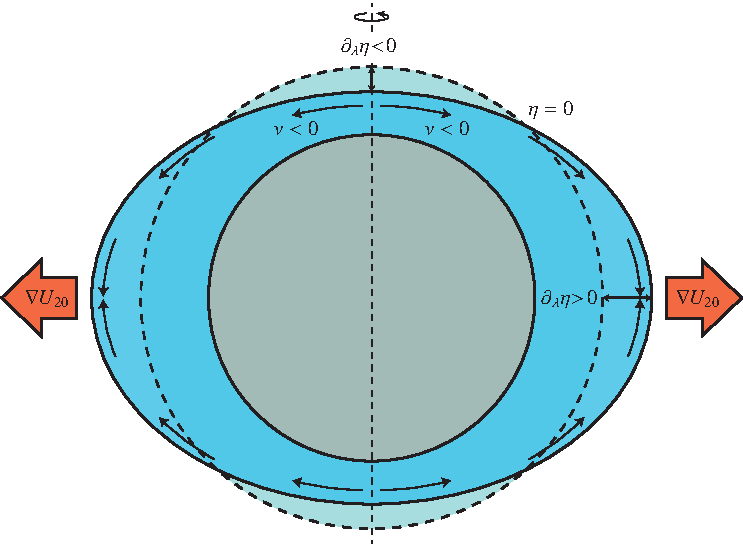
\includegraphics[width=0.7\linewidth]{Figures/CoordProb}
\caption{Schematic representation of the ocean tide due to the eccentricity-radial tidal potential ($U_{20}$), at periapsis. Taking the derivative of $v$ across the north pole yields a zero result in the spherical coordinate system, despite the clear mass divergence away from the poles which should result in $\partial_{\lambda} \eta < 0$.\label{fig:coord_prob}}
\end{figure}

A more significant issue arises from the combined choice of coordinate system and grid structure. Nodes located directly at the poles become singularities in space, as the normal directions east and west used to define the velocity components become meaningless. Consider the northward velocity flow near the north pole under the eccentricity-radial tide, shown in Figure \ref{fig:coord_prob}. Conservation of mass and the formation of an equatorial bulge force flow to diverge away from the pole. In solving for the surface displacement node directly at $\lambda = 90^{\circ}$, we must take the derivative of $v$ across the pole (as in Equation \ref{eq:momv_fd}). As each $v$ node located either side of the pole has the same magnitude and, perhaps unintuitively, is orientated in the same direction (southwards), this derivative becomes zero.  This forces surface displacement at the pole to zero as well. Yet, as there is divergence away from the pole, it is required that $\partial_{\lambda} \eta < 0$ to conserve mass. Clearly, the choice of coordinate system and grid do not permit such behaviour at the poles. 

To work around this problem, we employ both first-order accurate one dimensional Euler interpolation and third-order accurate Lagrange interpolation for all $u$ and $\eta$ nodes located at the pole, avoiding the need to directly solve for these points. We then take the mean of the interpolated $\eta$ points and prescribe that as the polar value. For $u$, the mean is taken for the eccentricity tide as eastward velocity tends towards zero at the poles. Average velocity is not computed for the obliquity tide, however, as non-zero eastward velocity components exist at the poles.

\subsection{Model Runs and Parameters \label{subsec:param}}

\begin{table}[!t]
\scriptsize
\centering
\begin{tabularx}{\linewidth}{p{1.5cm} p{2.5cm} p{2.5cm}}
 \toprule
Parameter & Description & Value\\
 \midrule \midrule
$\Omega$ & angular velocity & $4.55 \times 10^{-6} \, \si{\radian\per\second}$\\
$r$ & satellite radius & $2574.7 \, \si{\kilo\metre}$\\
$a$ & semi-major axis & $1.221865 \times 10^6 \, \si{\kilo\metre}$\\
$g$ & surface gravity & $1.35 \, \si{\metre\per\second\squared}$\\
$e$ & eccentricity & $0.0288$\\
$\theta_0$ & obliquity & $0.32^{\circ}$\\
$k_2$ & tidal Love number & $0.120$\\
$h_2$ & tidal Love number & $0.2$\\
 \bottomrule
\end{tabularx}
\caption{Model parameters used in all simulations presented here. All values are specific to Titan, and are taken from \citet{zebker2009size,chen2013tidal}.  \label{tb:param}}
\end{table}

We first perform both semi-analytical and numerical simulations for Titan and Enceladus under the eccentricity and obliquity tides. For each tidal component over 3000 simulations were run for \hbox{$h_0 = 1 - 10^4 \, \si{\metre}$} and \hbox{$\alpha = 10^{-9} - 10^{-5} \, \si{\per\second}$}. Such resolution is necessary to capture resonant features. The semi-analytical solution for the time averaged surface heat flux from \citet{matsuyama2014tidal} was directly compared to the numerical values to reveal any inaccuracies in the numerical solution across this parameter space. 

Following testing and verification of the numerical solutions for Rayleigh drag, ODIS was then run using only bottom drag for \hbox{$h_0 = 1 - 10^4 \, \si{\metre}$} and \hbox{$c_D = 10^{-7} - 10^{-1}$}. These simulations were again run for both the eccentricity and obliquity tides. With results for both Rayleigh and bottom drag we were able to compare tidal dissipation between these two drag regimes. The model parameters used for both Titan and Enceladus are shown in Table \ref{tb:param}.

Numerically solving the LTEs to convergence is a computationally expensive process. As shown in Figure \ref{fig:conv_a}, convergence will only be reached after a significant amount of simulation time. The example given in Figure \ref{fig:conv_a} was run using initial conditions for a stationary, undisturbed ocean. To speed up convergence we employ the technique used by \citet{sears1995tidal}, whereby the final output of one simulation is used as the initial condition for the next simulation. Upon completion, each simulation will spawn one to two `child' simulations. These new simulations will in turn spawn their own `children' once they are complete. This method of solving over such a large parameter space helps to significantly reduce computational run and spin-up time. Several tests were also run to ensure that a given simulation would converge to a single solution, regardless of initial condition.





\begin{figure*}[!t]
    \centering
    \begin{subfigure}[t]{0.85\linewidth} % contains the two plots in a single figure
        \includegraphics[width=\linewidth]{Figures/titan_linear}
        \phantomcaption
        \label{fig:lincEccTitan}
    \end{subfigure}
    \begin{subfigure}[t]{0\linewidth} % the hidden unwanted image
         \includegraphics[width=\linewidth]{Figures/titan_linear}
         \phantomcaption
         \label{fig:linObliqTitan}   
    \end{subfigure}
    \vspace{-0.5cm}
\caption{Global ocean surface dissipation solution for Titan under the eccentricity (left) and obliquity (right) tides. The logarithm of dissipated energy is shown as a function of ocean depth, $h$, and Rayleigh drag coefficient, $\alpha$. All simulations were performed with \SIrange{2}{3}{\degree} resolution.}
\label{fig:linTitan}
\end{figure*}

\section{Ocean Dissipation in Titan \label{sec:results_Titan}}

The following results are split into three main sections. Firstly, we compare dissipation between Rayleigh (section \ref{sec:ray_titan}) and bottom (section \ref{subsec:botTitan}) drag for Titan. Section \ref{subsec:scalTitan} then compares the bottom drag results to scaling laws from \citet{chen2013tidal}. We repeat these results for Enceladus in section \ref{sec:results_Enceladus}.

\subsection{Rayleigh Drag}\label{sec:ray_titan}

Dissipated surface heat flux averaged over the tidal period was calculated for over 3000 simulations over $h$ and $\alpha$ space for each main tidal component, as shown in Figure \ref{fig:linTitan}. The eccentricity tide (Figure \ref{fig:lincEccTitan}) shows three resonant ocean thicknesses, $h \sim$ \SIlist{2;3;22}{\metre}. These horizontal resonances are the result of excited gravity waves, with the deepest of these having a maximum dissipated surface heat flux of $\sim 10\, \si{\watt\per\square\metre}$ which occurs between $\alpha =$ \SIrange{e-8}{e-7}{\per\second}. Notably, the maximum dissipated energy does not occur for the most drag dominated oceans where $\alpha \sim \num{e-5} \, \si{\per\second}$. 

\begin{figure*}[!t]
    \centering
    \begin{subfigure}[t]{0.85\linewidth} % contains the two plots in a single figure
        \includegraphics[width=\linewidth]{Figures/titan_bottom}
        \phantomcaption
        \label{fig:botEccTitan}
    \end{subfigure}
    \begin{subfigure}[t]{0\linewidth} % the hidden unwanted image
         \includegraphics[width=\linewidth]{Figures/titan_bottom}
         \phantomcaption
         \label{fig:botObliqTitan}   
    \end{subfigure}
    \vspace{-0.5cm}
\caption{Global ocean surface dissipation solution for Titan under the eccentricity (left) and obliquity (right) tides. The logarithm of dissipated energy is shown as function of ocean depth, $h$, and coefficient of bottom drag, $c_D$. All simulations were performed with \SIrange{1}{3}{\degree} resolution. \label{fig:botTitan}}
\end{figure*}


Figure \ref{fig:linObliqTitan} illustrates the dissipated surface heat flux for the obliquity tide on Titan. Two resonant ocean thicknesses are found for this tidal component, $h \sim$ \SIlist{1;10}{\metre}. The latter resonance is the most dissipative with an average surface heat flux of $\sim \num{4e-3}\, \si{\watt\per\square\metre}$. There is also an excited Rossby wave resonance orientated diagonally across $h \sim$ \SIrange{10}{e4}{\metre} and \hbox{$\alpha \sim$ \SIrange{e-6}{e-9}{\per\second}}. The average surface heat flux occurring along the length of this resonance is $\sim \SI{e-4}{\watt\per\square\metre}$. 

Numerical error was also computed using the semi-analytical solutions from \citep{matsuyama2014tidal}. The eccentricity tide is accurate to within 1\% over much of the parameter space, with resonances being the least accurate (in terms of absolute value). The deepest resonance differs from the analytical solution by \SIrange{1}{20}{\percent}. We ignore discrepancies in shallow oceans ($h_0 \leq 10 \, \si{\metre}$) as bathymetry of the ocean floor for any icy satellite will likely be comparable to or exceed the depth of such a thin the ocean, directly violating the assumptions made in the LTEs. It should also be noted that resonances found below $h_0 = 10 \, \si{\metre}$ typical have displacements greater than the depth of the ocean itself, another violation of the LTEs assumptions. As such, we deem this part of the parameter space unphysical.

\subsection{Bottom Drag \label{subsec:botTitan}}

Dissipation across $h$ and $c_D$ space (bottom drag) is shown in Figure \ref{fig:botTitan}. Tidal dissipation due to the eccentricity tide is shown in the left hand figure. Comparing this to Rayleigh dissipation in Figure \ref{fig:lincEccTitan} highlights some of the major differences and similarities between the two drag regimes. The resonant peaks at \SIlist{2;3;22}{\metre} from the Rayleigh drag case are all present, although they have smaller magnitudes. The resonance broadens towards larger $c_D$, and remains very diffuse over much of the parameter space. This differs from the Rayleigh drag case where the resonances are very narrow and pronounced over most of $\alpha$ space (Figure \ref{fig:lincEccTitan}). Additionally, away from the resonances and in the deepest oceans, dissipated energy drops by \numrange{10}{12} orders of magnitude when applying bottom drag, which is far smaller than the lowest dissipation found in the Rayleigh drag case.  

Ocean dissipation under the obliquity tide using bottom drag also has several important differences and similarities to the Rayleigh case. Comparing figures \ref{fig:botObliqTitan} and \ref{fig:linObliqTitan}, it is again evident that the horizontal gravity wave resonances at \SIlist{1;10}{\metre} are present in both solutions. Perhaps the most significant difference between each case is the orientation of the broad resonance that extends to the deepest oceans. In the Rayleigh case, this resonance moves diagonally across a large region of the parameter space, whereas it is vertically oriented and limited to a small range of $c_D$ for the bottom drag case, such that the resonance becomes independent of ocean depth. The resonance also happens to occur across the empirically derived Earth value for $c_D = 0.002$ \citep[e.g.,][]{sohl1995tidal,egbert2001estimates}. %Unlike in the Rayleigh case, these resonances rapidly broaden towards higher $c_D$, when bottom drag becomes more dominant

\subsection{Comparison with Scaling Laws \label{subsec:scalTitan}}

\begin{figure*}[!t]
\centering
\begin{subfigure}{0.5\linewidth}
\centering
\includegraphics[width=0.85\linewidth]{Figures/Eccentricity_scaling}
\subcaption{\label{fig:scalEccTitan}}
\end{subfigure}%
\begin{subfigure}{0.5\linewidth}
\centering
\includegraphics[width=0.85\linewidth]{Figures/Obliquity_scaling}
\subcaption{\label{fig:scalObliqTitan}}
\end{subfigure}
\vspace*{-0.8cm}
\caption{Comparison of the ODIS numerical results (solid lines) and those calculated using the scaling laws (dashed lines) derived in \citet{chen2013tidal}, for Titan under the eccentricity (left) and obliquity (right) tides.\label{fig:scalTitan}}
\end{figure*}

While there are no fully analytical solutions to the LTEs when including bottom drag, there are a set of scaling laws for estimating dissipation that neglect gravity wave resonant features, developed by \citet{chen2013tidal}. We compare cross sections from the results in Figure \ref{fig:botTitan} with these scaling laws, shown in Figure \ref{fig:scalTitan}.

Away from resonances and in deep oceans, there is excellent agreement between the numerical results and the scaling laws. This is particularly true of the eccentricity tide. Larger discrepancies are found for the obliquity tide (Figure \ref{fig:scalObliqTitan}) for deep oceans, but this is a result of discretisation error. The vertically orientated resonant feature in Figure \ref{fig:botObliqTitan} is also produced from the scaling laws, as shown in Figure \ref{fig:scalObliqTitan}. None of the gravity wave resonances are captured by the scaling laws. 

\subsection{Implications for Titan}

Titan likely has an ocean that is several hundred kilometres thick \citep{sohl2003interior}. All of the eccentricity tide resonances occur at ocean depths much shallower than this, suggesting that - despite the substantial free eccentricity - there is little dissipation from this tidal component in heating Titan's ocean.

Rossby wave resonances from the obliquity tide appear as the diagonal and vertical features in figures \ref{fig:linObliqTitan} and \ref{fig:botObliqTitan}, respectively. The linear drag resonance moves into unrealistically low Rayleigh drag coefficients ($\alpha \lesssim$ \SI{e-9}{\per\second}) for oceans deeper than about \SI{10}{\kilo\metre}. However, for bottom drag, the Rossby wave resonance is mainly independent of ocean depth above $h \gtrsim$ \SI{1}{\kilo\metre}. If Titan's ocean fell within the $c_D =$ \SIrange{e-2}{e-4} range then this Rossby wave resonance could provide a non-neglible thermal energy component to Titan's interior, regardless of the ocean depth. To gain some insight into how significant this dissipation can be, we consider some upper limits of Titan's semimajor axis evolution.

Hyperion is the next furthest satellite from Saturn after Titan, with a semimajor axis  \num{1.21} times that of Titan's \citep{sears1995tidal}. Titan would had to have originated at some semimajor axis less than Hyperion's, otherwise Hyperion would have been disturbed or ejected from the system, assuming Hyperion and Titan have similar ages. This provides us with a useful upper bound on Titan's  initial semimajor axis. Using the dissipated energy results for the obliquity tide under bottom drag we can examine how rapidly Titan's semimajor axis shrinks to its present day value.

For a bound orbit the total energy is given as $-GMm/2a$ \citep{goldreich1966q}. Differentiating this expression with respect to time gives a relationship between the dissipated energy and changing semimajor axis,
\begin{equation}
\dot{a} = \dfrac{2a^2 \dot{E}}{GM m}.
\label{eq:adot}
\end{equation}

where $M$ and $m$ represent the mass of Saturn and Titan, respectively. The universal gravitational constant is $G$, and dissipated energy in watts is $\dot{E}$. Note that as $\dot{E} < 0$, the semimajor axis decays with time. To first order, we find that $\dot{E}$ remains nearly constant over the range $1.21 a$ to $a$ for a deep ocean on Titan experiencing bottom drag for the obliquity tide. This is because the position of the vertical Rossby wave resonance (Figure \ref{fig:botObliqTitan}) is sensitive to the rotation rate of Titan, which hardly varies from $\Omega =$ \SIrange{4.56e-6}{3.42e-6}{\per\second} over the range of semimajor axes that we consider, assuming synchronous rotation. We are thus able to set $\dot{E}$ to constant in the following calculations. Additionally, it should be noted that while $\dot{E}$ is rather sensitive to the actual obliquity, $\theta_0$, we set the obliquity to constant over time for simplicity. A more rigorous (and future) approach would include the coupling between dissipation energy and obliquity.

\begin{figure}[!b]
\centering
\includegraphics[width=\linewidth]{Figures/titan_timescale}
\caption{Semimajor axis decay timescale, $\tau_a$, as a function of ocean depth and bottom drag coefficient for the obliquity tide on Titan. This timescale represents the time taken for the semimajor axis of Titan to shrink from that of Hyperion's to the present day value. \label{fig:a_evo}}
\end{figure}

\begin{figure*}[!t]
    \centering
    \begin{subfigure}[t]{0.85\linewidth} % contains the two plots in a single figure
        \includegraphics[width=\linewidth]{Figures/enceladus_linear}
        \phantomcaption
        \label{fig:lincEccEncel}
    \end{subfigure}
    \begin{subfigure}[t]{0\linewidth} % the hidden unwanted image
         \includegraphics[width=\linewidth]{Figures/enceladus_linear}
         \phantomcaption
         \label{fig:linObliqEncel} 
    \end{subfigure}
    \vspace{-0.5cm}
\caption{Time and surface averaged ocean dissipation for Enceladus under the eccentricity (left) and obliquity (right) tides when applying Rayleigh drag. The logarithm of dissipated energy is shown as function of ocean depth, $h$, and bottom drag coefficient, $c_D$. All simulations were performed with \SIrange{1}{3}{\degree} grid resolution. \label{fig:linEncel}}
\end{figure*}

We integrate Equation \ref{eq:adot} to estimate the evolution of Titan's semimajor axis as a function of time and dissipated energy, defining a characteristic semimajor axis decay time, $\tau_{a}$, as the time taken for the semimajor axis to reach its present day value from Hyperion's. The decay time as a function of ocean depth and bottom drag coefficient is shown in Figure \ref{fig:a_evo}.
  
As expected, the smallest $\tau_a$ occurs for the largest dissipation, namely the gravity wave resonance at \SI{10}{\metre}, with decay times on the order of \SIrange{10}{100}{\mega\year}. However, as previously mentioned, Titan's ocean is likely in excess of \SI{100}{\kilo\metre} thick, and is thus far from this resonance. Figure \ref{fig:a_evo} shows that for ocean depths $h_0 >$ \SI{1}{\kilo\metre} the decay time-scale (and dissipation) is effectively independent of ocean depth. Although not shown, this behaviour continues right up to the shallow water limit ($h_0 \lesssim 0.1r$) as predicted by the \citet{chen2013tidal} scaling laws. Thus, for $c_D =$ \SIrange{e-4}{2e-2}, Titan's semimajor axis would shrink to its present day value in less than the age of the Solar System ($\sim$\SI{4.5}{\giga\year}, denoted by the dashed contour in Figure \ref{fig:a_evo}). If Titan's orbit originated with a semimajor axis between its current value and less than Hyperion's value, then we would expect Titan to have a smaller semimajor axis than that observed today.

Although the initial value of $a$ is not known, the scenario described above is not consistent with the deep ocean estimates of \citet{sohl2003interior} if we assume a bottom drag coefficient within an order of magnitude of the canonical Earth value ($c_D =$ \num{0.002}). Instead, our estimates of the decay time-scale suggest that Titan's ocean has a bottom drag coefficient of \hbox{$ \num{e-4} \gtrsim c_D \gtrsim \num{2e-2} $}. These constraints indicate that Titan's ocean experiences anomalously low or high drag (not dissipation) than compared to the Earth's ocean.

The authors find it possible to argue for either the high or low drag limit. Titan is a very slow rotator, resulting in limited ocean flow. This factor reduces the amount of turbulent bottom flow experienced in the ocean, consequently lowering the bottom drag coefficient. This is consistent with the low drag limit. However, one could additionally argue that the presence of a solid lid, although neglected here, would result in an extremely turbulent ``top'' drag environment, consistent with the high drag limit. At present there is not sufficient evidence to favour one of these limits over the other and should be a focus of future work.  

Although we do not attempt to compute the eccentricity evolution (which is far more challenging with non-radial tidal components), the almost negligible amount of dissipated energy for $h_0 >$ \SI{1}{\kilo\metre} shown in Figure \ref{fig:botObliqTitan} should allow Titan to maintain its relatively high free eccentricity of 0.0288. Here we of course neglect dissipation in Titan's solid interior.
\section{Ocean Dissipation in Enceladus \label{sec:results_Enceladus}}

\subsection{Rayleigh Drag} \label{sec:ray_enc}

As with our Titan results, we calculated globally averaged surface heat flux for over 3000 simulations in the $h$-$\alpha$ parameter space. These results are shown for the eccentricity and obliquity tides in Figure \ref{fig:linEncel}.

There are several more gravity wave resonances found for Enceladus than Titan in both tidal components, as shown in Figure \ref{fig:lincEccEncel}. The eccentricity tide excites resonances at \SIlist{1.3;1.9;3.8;8.7;29;50;360}{m}; a total of 7 resonances, whereas Titan only has 3 (Figure \ref{fig:lincEccTitan}). 
%By solving the LTEs using both the eccentricity-radial and libration tides simultaneously, we capture any coupling these two tidal components may initiate in the ocean flow and find no new resonances. 
Increasing the resolution of the parameter space would almost certainly reveal more resonances, but this is only likely for oceans with $h_0 <$ \SI{10}{\metre}. As is the case with the Titan results in section \ref{sec:results_Titan}, we again find excellent agreement between the numerical and semi-analytical solutions of \citet{matsuyama2014tidal} over the majority of the explored parameter space. The ocean resonances are found at the same ocean thickness in both solutions, with only their magnitudes exhibiting up to \SI{10}{\percent} difference for the deepest resonance.

The most dissipative eccentricity tide resonance is also the deepest, with an average surface heat flux of \SI{4.6}{\watt\per\square\metre} at $\alpha\sim$ \SI{2e-6}{\per\second}, three orders of magnitude more dissipative than Titan's largest resonance. This is equivalent to a total power output of $\sim$ \SI{3610}{\giga\watt}, well in excess of the observed value of (at least) \SI{5}{\giga\watt} by two to three orders of magnitude \citep{spencer2006cassini,howett2011high, spencer2013new}.  

\begin{figure}[!t]
    \centering
    \includegraphics[width=\linewidth]{Figures/enceladus_bottom}
\caption{As for Figure \ref{fig:linEncel}, but for the bottom drag regime. The obliquity tide is also ignored. \label{fig:botEncel}}
\end{figure}

The stark colour difference between the eccentricity and obliquity tide plots in Figure \ref{fig:linEncel} is a result of Enceladus' negligible obliquity ($\theta_0 \sim$ \num{e-4} degrees \citep{chen2013tidal, baland2016obliquity}). This causes average surface dissipation to range from \SIrange{e-7}{e-14}{\watt\per\square\metre} over our explored parameter space, which has an almost negligible effect on the thermal and orbital evolution of the satellite. Gravity wave resonances are found at \SIlist{1.6;2.7;5.5;18;160}{\metre}, with the characteristic Rossby wave resonance extending diagonally across the parameter space from around $h=$ \SI{500}{\metre}.

Away from shallow oceans, we once again find excellent agreement between the numerical and semi-analytical solutions from \citet{matsuyama2014tidal} in terms of both the resonant ocean thicknesses and magnitude of the dissipation. Much of the parameter space has a discrepancy of $<$ \SIrange{1}{5}{\percent}, with this increasing to $\sim$ \SI{10}{\percent} for resonances. As demonstrated in Figure \ref{fig:conv}, this can easily be decreased with higher resolution simulations, at the expense of computational run time.


\subsection{Bottom Drag}

We neglect running the obliquity tide bottom drag case for Enceladus. As mentioned in the previous section, the obliquity of Enceladus is close to Cassini state \citep{chen2011obliquity,chen2013tidal}, making tidal flow and dissipation from obliquity negligible. Additionally, the low drag experienced due to weak obliquity tide flow leads to long simulation run times in order to achieve equilibrium, which is a severe challenge numerically.

Bottom drag results for the eccentricity tide on Enceladus are shown in Figure \ref{fig:botEncel}. The gravity wave resonances are found at identical ocean thicknesses to the Rayleigh drag results in Figure \ref{fig:lincEccEncel}. There is, however, a much greater contrast in dissipation magnitude in this parameter space when compared to the Rayleigh drag results. Dissipation drops off rapidly by many orders of magnitude with increasing ocean depth away from the \SI{360}{\metre} resonance. This is expected given the velocity squared dependence in the bottom drag term in Equation \ref{eq:mom}. 

\subsection{Comparison with Scaling Laws}

\begin{figure}[!b]
\centering
\includegraphics[width=0.85\linewidth]{Figures/enceladus_scaling}
\caption{Comparison of the ODIS numerical results (solid lines) and those calculated using the scaling laws (dashed lines) derived in \citet{chen2013tidal}, for Enceladus under the eccentricity tide. The colours represent different values of bottom drag coefficient. \label{fig:scalEncel}}
\end{figure}

The bottom drag eccentricity tide results for Enceladus are compared to \citet{chen2013tidal} scaling laws in Figure \ref{fig:scalEncel}. As was the case with Titan, we find poor agreement for resonant ocean configurations, with increasingly good agreement away from resonances. The scaling laws cannot take into account the resonant ocean configurations due to the non-linearity of these features. However, the general trend of decreasing dissipation with increasing ocean depth is captured by the scaling laws and agrees well with our numerical results. This agreement provides further validation to the numerical model and techniques employed in this work.

\subsection{Implications for Enceladus}

Eccentricity is the only significant contributor to ocean dissipation in Enceladus. Under both Rayleigh and bottom drag, the deepest occurring gravity wave resonance can easily account for the observed SPT power output \citep{spencer2006cassini,howett2011high,spencer2013new}. However, this resonance is relatively shallow. Of course, Enceladus' ocean depth is unconstrained, although non-unique gravity modelling is consistent with an ocean on the order of \SI{10}{\kilo\metre} thick, at least under the SPT \citep{iess2014gravity}. Thus, based on our results, we expect that ocean dissipation is insignificant over long time scales for Enceladus. 
%Resonant ocean configurations occur only for shallow oceans under the eccentricity tide and obliquity tide flow is negligible, meaning dissipation is minimal over the vast majority of the likely parameter space.

%The numerical model has also revealed no new resonances in either Rayleigh or bottom drag by applying both the eccentricity-radial and eccentricity-libration tide simultaneously, a technique that is not possible analytically.

The amplitude of forced libration on Enceladus \citep{thomas2015enceladus}, as well as the negative mass anomaly observed at the SPT \citep{iess2014gravity, mckinnon2015effect} indicate that its subsurface ocean is global in extent and deeper beneath the SPT. This variable ocean thickness is neglected in our model, and may lead to localised heating at the boundary between shallow and deep oceans. The effect on resonance ocean configurations is unknown. Incorporating a variable ocean thickness into the LTEs is only possible numerically, and will be one focus of future work.


%\section{Discussion \label{sec:discussion}}

\subsection{Considering Tidal Q \label{sec:Q}}


\section{Conclusions}

We have designed and implemented a numerical model based on \citet{sears1995tidal} to solve the dissipative Laplace Tidal Equations on a sphere. This model, valid only in the shallow water limit and assuming a global surface ocean, has been used to model ocean flow and its associated tidal dissipation over a range of ocean thickness and drag coefficients for both Titan and Enceladus. We neglect the effects of ocean loading and self-attraction.

Modelling is performed with both Rayleigh (linear) and bottom (quadratic) drag models. The former represents internal drag between two adjacent fluid parcels \citep{neumann1968ocean}, while the latter is a global scale approach to incorporating the effects of a macro-scale turbulent boundary layer at some solid-fluid interface \citep{gill1982atmosphere}.

Rayleigh drag results were compared to that of \citet{matsuyama2014tidal} yielding mostly excellent agreement over much of the explored parameter space, providing important validation to our numerical model. The presence and position of ocean dissipative resonances were replicated well in both Rayleigh and bottom drag simulations. Importantly, we have also demonstrated good agreement between our bottom drag numerical results and the scaling laws of \citet{chen2013tidal} away from gravity wave resonances, providing further validation of the bottom drag implementation in our model.

For Titan, we found that the Rossby wave resonance associated with the obliquity tide becomes independent of ocean depth away from shallow ($h \sim\SI{1}{\kilo\metre}$) oceans. This is also shown in the \citet{chen2013tidal} obliquity tide scaling law. Such depth independence allows us to place loose constraints on the bottom drag coefficient in Titan's ocean by modelling semimajor axis evolution under the assumption of a deep ocean \citep{sohl2014structural,baland2014titan}. We find that bottom drag coefficients of less that \SI{e-4} or greater than \SI{2e-2} are acceptable to recreate Titan's present day semimajor axis, assuming a starting semimajor axis equal to Hyperion's (the next outer satellite of Saturn). Both limits are an order of magnitude away from the canonical Earth value ($\sim 0.002$ \citep{egbert2001estimates}), indicating that Titan has either anomalously low or high drag in its ocean. We currently cannot distinguish between these two regimes. 

Enceladus' eccentricity tide ocean resonances are found to be extremely dissipative, as in \citet{tyler2011tidal, matsuyama2014tidal}. However, the ocean depths associated with the deepest of these resonances are too shallow to be a probable scenario on Enceladus. We hope to model tidal flow for a spatially varying ocean thickness on Enceladus in the future, as this will likely effect resonant thicknesses and may lead to more localised heating at the SPT. Additionally, it is important to incorporate the effects of an icy shell atop these oceans to understand how this limits ocean dynamics and dissipation, which will be explored in future work. 

\section*{References}
\bibliography{mybibfile}

%\appendix

\section{Laplace Tidal Equations in Spherical Coordinates \label{app:coords}}

To convert the Laplace Tidal Equations to a spherical coordinate system we must make use of the following well-known identities for the gradient and divergence operators,
\begin{equation}
\nabla f = \frac{1}{R} \partial_{\lambda} f \bm{\hat{\lambda}}  
+ \frac{1}{R \cos{\lambda}} \partial_{\lambda} f \bm{\hat{\phi}}
\end{equation}
\begin{equation}
\nabla \cdot \bm{A} = -\frac{1}{R \cos{\lambda}} \partial_{\lambda} \left( \cos{\lambda}\, A_{\lambda} \right) + \frac{1}{R \cos{\lambda}} \partial_{\phi} A_{\phi}
\end{equation}

where $\bm{A}$ is some vector quantity tangent to the spherical surface, $f$ is a scalar quantity, and $\bm{\hat{\lambda}}$ and $\bm{\hat{\phi}}$ are the latitude and longitude unit vectors, also tangent to the surface. Note that we ignore any component of the divergence and gradient operators in the radial direction in accordance with the shallow water assumptions.

Defining $\bm{u} = \left(u, v \right) = (u_{\phi}, -u_{\lambda} ) $ and using the fact that $\bm{\Omega} = \Omega \bm{\hat{k}}$, where $\bm{\hat{k}}$ is the Cartesian unit vector aligned with the rotation axis, then the continuity equation can be rewritten as,
\begin{equation}
\partial_t \eta + \frac{h_0}{R \cos{\lambda}} \left( \partial_{\lambda}
\left(v \cos{\lambda} \right) +  \partial_{\phi} u \right) = 0 \, .
\end{equation}

\noindent Similarly, the momentum equation becomes, 
\begin{equation}
\partial_t u - 2 \Omega v \sin{\lambda}
+ \alpha u
+\frac{c_D}{h_0} \left(u^2 + v^2 \right)^{\nicefrac{1}{2}} u
+ \frac{g}{R \cos{\lambda}} \partial_{\phi} \eta
= 
(1 + k_2 - h_2) \frac{1}{R \cos{\lambda}} \partial_{\phi} U_2
\end{equation}
\begin{equation}
\partial_t v + 2 \Omega u \sin{\lambda}
+ \alpha v
+\frac{c_D}{h_0} \left(u^2 + v^2 \right)^{\nicefrac{1}{2}} v
+ \frac{g}{R} \partial_{\lambda} \eta
= 
(1 + k_2 - h_2) \frac{1}{R} \partial_{\lambda} U_2
\end{equation}

%
%\section{Finite Difference Energy Expressions \}
%
%For a system experiencing both Rayleigh and bottom friction, the full dissipated energy over an orbit is given by,
%\begin{equation}
%F = \frac{\rho}{4 \pi T} \iint \left[h \alpha \left(u^2 + v^2 \right) + c_D \left(u^2 + v^2 \right)^\nicefrac{3}{2} \right}d\Omega dt,
%\end{equation}
%
%\noindent where $\Omega$ is the solid angle and we assume that $h \ll R$.


\section{Numerical Error and Testing \label{app:error_tests}}

\textbf{This appendix outlines how numerical error was quantified in this study, as well as several numerical tests that were performed to benchmark our code.}

\textbf{Numerical error is quantified in two distinct ways in this manuscript. Local error, such as that plotted in Figure \ref{fig:spatial_error}, is simply calculated as the percentage error:}
\begin{equation}
E_i = \dfrac{\left| x_{i, num} - x_{i, anlyt} \right| }{x_{anlyt}} \times 100 \, .
\end{equation}

To investigate global error at a particular simulation time, such as that shown in figures \ref{fig:temporal_error} and \ref{fig:spatial_convergence}, we use the normalised $L_1$, $L_2$, and $L_{\infty}$ error norms:
\begin{align}
L_1 &= \dfrac{1}{N}\sum_1^N \left| x_{i, num} - x_{i, anlyt} \right| \, , \\
L_2 &= \left( \dfrac{1}{N}\sum_1^N \left| x_{i, num} - x_{i, anlyt} \right|^2 \right)^{\nicefrac{1}{2}}\, , \\
L_{\infty} &= \text{max} \left| x_{i, num} - x_{i, anlyt} \right|\, ,
\end{align}

\textbf{\noindent where $N$ is the total number of grid points in the model domain, and $i$ is the index of each cell. The normalised approach is common in CFD problems as it allows one to estimate the convergence order of the implemented numerical method.}

As with any numerical solution there are errors associated with discretisation of the problem into the model domain. We performed resolution testing across various ocean thicknesses to determine how these errors scale with grid resolution \textbf{using the semi-analytical solutions of \citet{matsuyama2014tidal} as our benchmark. Although the solutions from \citet{matsuyama2014tidal} are not purely analytical, we use solutions that are truncated at spherical harmonic degree $l=30$. As such, these can be considered the exact solutions. Four of these tests are shown in this section to illustrate that the numerical method and code perform as expected, both as a function of space and time. Tests \numrange{1}{3} were run for Enceladus' eccentricity tide, using $h_0 = \SI{500}{\metre}$, $\alpha = \SI{e-5}{\per\second}$, and $\Delta t = \SI{2}{\second}$. Test 4 was for the obliquity tide on Titan using $h_0 = \SI{1}{\kilo\metre}$ and $\alpha = \SI{e-8}{\per\second}$. The grid was spaced at \SI{1}{\degree} throughout, except in tests 3 and 4 which examine how the numerical error depends on model resolution.}

\begin{figure}
\centering
\includegraphics[width=0.85\linewidth]{Figures/spatial_error_ecc}
\caption{\textbf{Displacement solutions (left column) and corresponding percentage error (right column) for Enceladus' eccentricity tide with $h_0 = \SI{500}{\metre}$ and $\alpha = \SI{e-5}{\per\second}$. The numerical grid was spaced at \SI{1}{\degree}. Each row corresponds to a different time interval throughout one orbital period, $T$. Percentage eror is  $< \SI{0.01}{\percent}$ over much of the model domain, with local highs where the solution passes from postive to negative displacement.} \label{fig:spatial_error}}
\end{figure}


\begin{figure}[t]
\centering
\includegraphics[width=\linewidth]{Figures/temporal_error_ecc}
\caption{\textbf{Normalised error norms as a function of time for Enceladus' eccentricity tide with $h_0 = \SI{500}{\metre}$ and $\alpha = \SI{e-5}{\per\second}$. At approximately \num{10} orbits, all parts of the solution have converged after which the normalised error remains small, and oscillates over the orbital period.} \label{fig:temporal_error}}
\end{figure}


\begin{figure}[t]
\centering
\includegraphics[width=0.6\linewidth]{Figures/convergence_eta}
\caption{\textbf{Normalised error norms as a function of time for Enceladus' eccentricity tide with $h_0 = \SI{500}{\metre}$ and $\alpha = \SI{e-5}{\per\second}$, taken at pericenter at the beginning of orbit \num{100}. A least-squares fit to each error norm in log-log space yields slopes of \num{0.86}, \num{0.90} and \num{1.03} for the $L_1$, $L_2$ and $L_{\infty}$ normalised error norms, respectively.} \label{fig:spatial_convergence}}
\end{figure}



\begin{figure*}[!t]
    \centering
    \begin{subfigure}[t]{\linewidth} % contains the two plots in a single figure
        \includegraphics[width=\linewidth]{Figures/convergence2}
        \phantomcaption
        \label{fig:conv_a}
    \end{subfigure}
    \begin{subfigure}[t]{0\linewidth} % the hidden unwanted image
         \includegraphics[width=\linewidth]{Figures/convergence2}
         \phantomcaption
         \label{fig:conv_b}   
    \end{subfigure}
    \vspace{-0.5cm}
\caption{Dissipation convergence and error scaling as a function of grid resolution. Panel \ref{fig:conv_a} shows the time evolution of the orbit-averaged dissipated energy at periapsis. The solid lines represents different grid resolutions, whereas the dashed line is the semi-analytical solution for Rayleigh drag from \citet{matsuyama2014tidal}. Panel \ref{fig:conv_b} shows the \textbf{dissipation} error between the numerical and semi-analytical solutions with increasing resolution. The least-squares slope of the first six data points (when the slope is steady) in log-log space is \num{1.94}. These simulations are for the obliquity tide using $h_0 = \SI{1}{\kilo\metre}$ and $\alpha = \SI{e-8}{\per\second}$ on Titan. \label{fig:conv}}
\end{figure*}

\textbf{It is important to understand how the model resolves the solution across the numerical domain, especially when using the fixed latitude-longitude grid employed here. This is done in test 1 (Figure \ref{fig:spatial_error}) where the ocean surface displacement (left) is compared to the corresponding error field (right). The ocean configuration is near a gravity-wave resonance, so it is easy to discern the eastward propagating gravity-wave through the model domain at each time slice. Percentage error in the numerical model is very small ($< \SI{0.01}{\percent}$) over the majority of the domain. Near the poles, where grid points are closely arranged, numerical error is smallest. At the zero-crossing in displacement both the numerical and semi-analytical solutions become $\ll \SI{1}{\metre}$. As a result, the numerical error locally spikes in those regions producing the rings of increased error seen in Figure \ref{fig:spatial_error}. Overall, the numerical error is very low, giving us confidence in the ability of ODIS to spatially resolve the solutions.}  

\textbf{As the tidal forcing in this problem is periodic, one expects the solution and its corresponding error to also be periodic. It is therefore logical to investigate how the numerical error changes over time. We investigate this in our second test, starting the numerical simulations from an undisturbed and unforced ocean. This is shown in Figure \ref{fig:temporal_error}, where once again the numerical error is computed against the \citet{matsuyama2014tidal} semi-analytical solutions. The error is quantified using the normalised $L_1$, $L_2$ and $L_{\infty}$ error norms, defined above. The maximum error in each solution is given by the $L_{\infty}$ norm. Normalised error is greatest at the beginning of the simulation, as this is during the model ``spin-up'' time. After approximately \num{10} orbits both the displacement and two velocity solutions converge. At this point the average error over each orbital period remains constant. The magnitude of this converged error is a function of the grid resolution, as shown in test 3. Once converged, the normalised error oscillates over the orbital period. This is expected; the maximum gradients in all three solutions periodically vary over an orbit. In regions where these gradients are maximised the finite difference scheme produces the poorest approximation. Consequently, the error varies as a function of time, even after convergence.  Although not shown, the simulation remains stable for over 1 year of simulation time. }

\textbf{In order to verify if the numerical scheme is implemented properly, it is prudent to perform convergence analysis on the numerical solutions. Figure \ref{fig:spatial_convergence} shows this analysis in our third test. The normalised error norms are plotted with varying grid resolution, spanning \SIrange{1}{10}{\degree} in both longitude and latitude. As expected, the accuracy of the numerical solution increases with decreasing grid size. With increasing resolution the local approximation of spatial derivatives improves, which is what produces this general trend. The rate at which the errors are reduced as a function of resolution is known as the order of convergence. This can be estimated by finding the slope of the normalised error norms in log-log space. Using a least-squares fit we find slopes of \num{0.86}, \num{0.90} and \num{1.03} for the $L_1$, $L_2$ and $L_{\infty}$ normalised error norms, respectively. We therefore conclude that the order of convergence of the numerical method implemented in ODIS is $\sim 1$, which is expected for the finite difference expansions made in equations \ref{eq:gen1} and \ref{eq:gen2}.}

\textbf{The total dissipated energy is of fundamental importance from the point of view of the Planetary Science community. As our final test we therefore investigate how the numerical dissipation solution varies as a function of time and grid resolution, shown in Figure \ref{fig:conv}. Unlike the other tests, this is run for the obliquity tide on Titan with an ocean of $h_0 = \SI{1}{\kilo\metre}$ and $\alpha = \SI{e-8}{\per\second}$. The numerical time- and orbit-averaged dissipated energy oscillates over time until converging to a single value, shown in the left panel. This final value gradually approaches the \citet{matsuyama2014tidal} semi-analytical solution as grid resolution is increased. The right panel, similar to Figure \ref{fig:spatial_convergence}, plots the numerical percentage error as a function of grid spacing. Again, the error decreases with decreasing grid spacing. The order of convergence for the dissipation is once again given by the slope of the line in Figure \ref{fig:conv_b}, which approaches $\sim 2$. As dissipated energy scales with the square of the velocity field, second order convergence is expected here.} 

Based on these resolution tests, all simulations were ran for grid resolutions of \SIrange{1}{3}{\degree} in latitude and longitude.

\end{document}
